\documentclass[14pt,final,oneside]{article}% класс документа, характеристики
%>>>>> Разметка документа
\usepackage[a4paper, mag=1000, left=3cm, right=1.5cm, top=2cm, bottom=2cm, headsep=0.7cm, footskip=1cm]{geometry} % По ГОСТу: left>=3cm, right=1cm, top=2cm, bottom=2cm,
\linespread{1} % межстройчный интервал по ГОСТу := 1.5
%<<<<< Разметка документа
\usepackage[utf8]{inputenc}
\usepackage[T2A]{fontenc}
\usepackage[english, russian]{babel}
\usepackage{amsmath, amsfonts, amssymb, amssymb, amsthm, mathtools}
\usepackage{geometry}
\usepackage{colortbl} % таблички
\usepackage{listings} % листинг
\usepackage{dcolumn} % выравнивание чисел
\usepackage[normalem]{ulem} % для подчёркиваний uline
\ULdepth = 0.16em % расстояние от линии до текста выше/ниже
\lstset{basicstyle=\ttfamily\normalsize}  
\usepackage{graphicx}
\usepackage{longtable}
\usepackage[breaklinks]{hyperref}
\usepackage{xcolor}
\usepackage{float}
\makeatletter
\def\cyrrange#1-#2{%
    \begingroup
    \count@=`#1
    \loop
    \lst@literate{\char\count@}{\char\count@}1
    \ifnum\count@<`#2
    \advance\count@\@ne
    \repeat
    \endgroup
}
\makeatother
\lstset{
    inputencoding=utf8,       % Указываем кодировку входного текста
    extendedchars=true,       % Включаем поддержку расширенных символов
    literate=%                % Настройка отображения кириллических символов
        {а}{{\selectfont а}}1
        {б}{{\selectfont б}}1
        {в}{{\selectfont в}}1
        {г}{{\selectfont г}}1
        {д}{{\selectfont д}}1
        {е}{{\selectfont е}}1
        {ё}{{\selectfont ё}}1
        {ж}{{\selectfont ж}}1
        {з}{{\selectfont з}}1
        {и}{{\selectfont и}}1
        {й}{{\selectfont й}}1
        {к}{{\selectfont к}}1
        {л}{{\selectfont л}}1
        {м}{{\selectfont м}}1
        {н}{{\selectfont н}}1
        {о}{{\selectfont о}}1
        {п}{{\selectfont п}}1
        {р}{{\selectfont р}}1
        {с}{{\selectfont с}}1
        {т}{{\selectfont т}}1
        {у}{{\selectfont у}}1
        {ф}{{\selectfont ф}}1
        {х}{{\selectfont х}}1
        {ц}{{\selectfont ц}}1
        {ч}{{\selectfont ч}}1
        {ш}{{\selectfont ш}}1
        {щ}{{\selectfont щ}}1
        {ъ}{{\selectfont ъ}}1
        {ы}{{\selectfont ы}}1
        {ь}{{\selectfont ь}}1
        {э}{{\selectfont э}}1
        {ю}{{\selectfont ю}}1
        {я}{{\selectfont я}}1
        {Б}{{\selectfont Б}}1
        {К}{{\selectfont К}}1
        {О}{{\selectfont О}}1
    language=Python,            % Язык программирования
    numbers=left,             % Нумерация строк слева
    stepnumber=1,             % Каждая строка нумеруется
    numbersep=5pt,            % Отступ от кода до номеров строк
    showspaces=false,         % Не показывать пробелы
    showstringspaces=false,   % Не показывать пробелы в строках
    tabsize=4,                % Размер табуляции
    frame=single,             % Рамка вокруг кода
    breaklines=true,          % Перенос строк
    breakatwhitespace=false,  % Переносить строки по пробелам
    basicstyle=\ttfamily,     % Шрифт текста
    keywordstyle=\color{blue},% Цвет ключевых слов
    commentstyle=\color{green},% Цвет комментариев
    stringstyle=\color{red},  % Цвет строковых литералов
}
\usepackage{minted} 

\usepackage{titlesec}
\titleformat{\section}
{\LARGE\bfseries}
{\thesection}{15pt}{} 
\usepackage{fancyhdr}
\renewcommand{\thesection}{\arabic{section}.}
\renewcommand{\thesubsection}{\arabic{section}.\arabic{subsection}.}
\usepackage{tocloft}
\renewcommand{\cftsecleader}{\cftdotfill{\cftdotsep}}
\renewcommand{\cftsecfont}{\Large\bfseries} 
\renewcommand{\cfttoctitlefont}{\LARGE\bfseries}
\newcommand{\lr}[1]{\left( {#1} \right)}
\usepackage{hyperref} % гиперссылки
\hypersetup{
    colorlinks=true,        % Включаем цветные ссылки
    linkcolor=blue!50!black, % Цвет внутренних ссылок (например, на разделы)
    urlcolor=blue!50!black,  % Цвет URL-ссылок
    citecolor=blue!50!black, % Цвет ссылок на библиографию
}
\usepackage{tikz}

% Команда для обведенного знака равенства
\newcommand{\circledequal}{%
    \mathbin{%
        \tikz[baseline=(X.base)] 
            \node[draw, circle, inner sep=0pt] (X) {$=$};%
    }%
}


\begin{document}
\thispagestyle{empty}
\begin{center}
\LARGE{Университет ИТМО} 
\vspace{20pt}

\vspace{180pt}

\LARGE{Длина кривой Безье\\
Евграфов Артём, 465826, P3109\\ 
Вариант 15 \\}
\vspace{335pt}
\end{center}

\begin{center}
\Large{Санкт-Петербург 2025}
\end{center}

\newpage
\setcounter{page}{1}
\noindent Протянуть оптоволоконный кабель от точки A до точки C, огибая точку K и используя наименьшее количество материала (длина кабеля минимальная). Для моделирования кабеля необходимо использовать единственную кривую Безье второго порядка на плоскости, проходящую через все три точки. В процессе решения нужно в явном виде использовать интегральную формулу вычисления длины кривой. Разрешается использовать любые программные пакеты для выполнения алгебраических операций и взятия интегралов, все вычисления следует привести в отчете с подробным описанием. В ответе должна присутствовать длина провода и координаты опорных точек кривой Безье. Также необходимо продемонстрировать результат графически. Кривая Безье второго порядка на плоскости имеет следующее уравнение: \\
\(B(t) = (1-t^2)A + 2t(1-t)B+t^2C\) — опорные точки кривой. A(0, 0); C(10, 0); K(3, 1). \\

\noindent Пусть $B(x_0, y_0)$ — неизвестная опорная точка, найдём её координаты. \\
\(x_K = (1-t_0)^2 x_A + 2t_0(1-t_0) x_B + t_0^2 x_C\) \\
\(y_K = (1-t_0)^2 y_A + 2t_0(1-t_0) y_B + t_0^2 y_C\) \\

\noindent Подставим известные значения: \\
\(3 = (1-t_0)^2 \cdot 0 + 2t_0(1-t_0) x_B + t_0^2 \cdot 10\) \\
\(x_B = \frac{3 - 10t_0^2}{2t_0(1-t_0)}\) \\

\noindent \(1 = (1-t_0)^2 \cdot 0 + 2t_0(1-t_0) y_B + t_0^2 \cdot 0\) \\
\(y_B = \frac{1}{2t_0(1-t_0)}\) \\

\noindent \(x(t) = (1-t^2)\cdot 0 + 2t\cdot(1-t)\cdot\frac{3-10t_0^2}{2t_0(1-t_0)}+t^2\cdot10 = t^2\left(10 - \frac{3-10t_0^2}{t_0(1-t_0)} \right) + t\cdot\frac{3-10t_0^2}{t_0(1-t_0)}, \; t_0 \in [0, 1]\)  \\
\(y(t) = (1-t^2)\cdot 0 + 2t\cdot(1-t)\cdot\frac{1}{2t_0(1-t_0)}+t^2\cdot0 = \frac{-t^2}{t_0(1-t_0)} + \frac{t}{t_0(1-t_0)}\) \\

\noindent Длину кривой посчитаем по формуле: \\
\[L = \int_0^1 \sqrt{\left( \frac{dx}{dt} \right)^2 + \left( \frac{dy}{dt} \right)^2} \, dt\]
\(\displaystyle \frac{dx}{dt} = 2t\left(10 - \frac{3-10t_0^2}{t_0(1-t_0)}\right) + \frac{3-10t_0^2}{t_0(1-t_0)}, \; \frac{dy}{dt} = \frac{-2t}{t_0(1-t_0)} + \frac{1}{t_0(1-t_0)}\) \\
\(\displaystyle L = \int_0^1 \sqrt{\left( \frac{dx}{dt} \right)^2 + \left( \frac{dy}{dt} \right) ^2} \, dt =  \int_0^1 \sqrt{\left(2t\left(10 - \frac{3-10t_0^2}{t_0(1-t_0)}\right) + \frac{3-10t_0^2}{t_0(1-t_0)}\right)^2 + \left(\frac{-2t}{t_0(1-t_0)} + \frac{1}{t_0(1-t_0)} \right)^2} \, dt = \) \\
\(\displaystyle=\frac{1}{t_0(1 - t_0)} \int_0^1 \sqrt{\left(2t(10t_0^2 + 10t_0 - 3) + (3 - 10t_0^2)\right)^2 + (1 - 2t)^2} \, dt\) \\
Методом бин поиска по ответам заметим, что минимум выражения достигается при $a \approx 0.3943, \; \displaystyle \int \approx 10.3099505958$. \\

\noindent Итого, координаты опорных точек: \(A(0, 0), \; B(3.0257, 2.0935), \; C(10, 0)\), а длина кабеля $ \approx 10.3099505958.$
\begin{figure}[H]
    \centering
    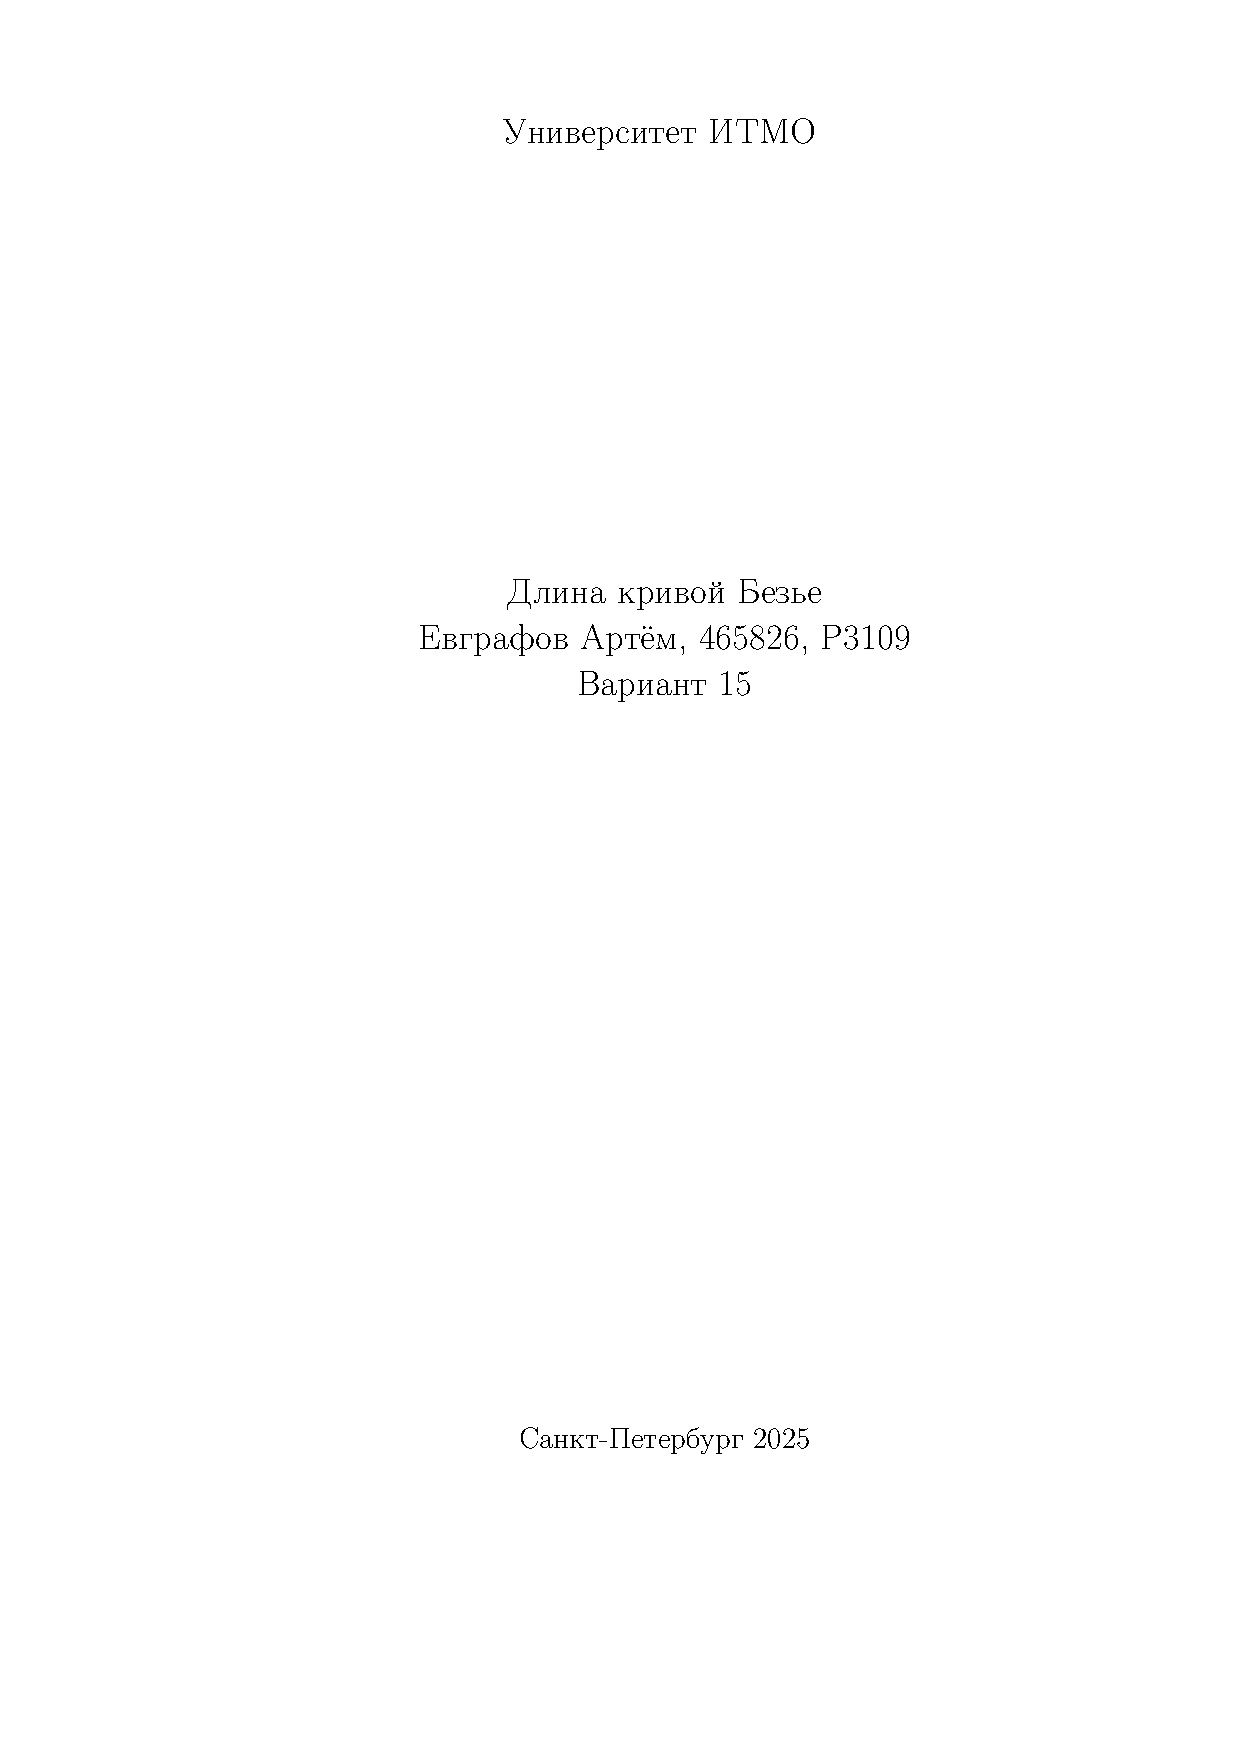
\includegraphics[width=0.8\linewidth]{bezye.png}
\end{figure}

\begin{minted}[linenos=true, frame=single, breaklines=true]{python}
import numpy as np
import matplotlib.pyplot as plt

A = np.array([0, 0])
B = np.array([3.0257, 2.0935])
C = np.array([10, 0])

def bezier(t, A, B, C):
    return (1-t)**2 * A + 2*t*(1-t) * B + t**2 * C

t = np.linspace(0, 1, 100)
curve = np.array([bezier(ti, A, B, C) for ti in t])

plt.figure(figsize=(8, 4))

plt.plot(curve[:, 0], curve[:, 1], label="Кривая Безье", color='blue')

plt.plot([A[0], B[0]], [A[1], B[1]], color='red', linestyle='--', label="Отрезок AB")
plt.plot([B[0], C[0]], [B[1], C[1]], color='green', linestyle='--', label="Отрезок BC")

plt.scatter([A[0], B[0], C[0]], [A[1], B[1], C[1]], color='red', label="Опорные точки")

plt.scatter([3], [1], color='purple', label="Точка K")

plt.legend()
plt.title("Кривая Безье")
plt.xlabel("X")
plt.ylabel("Y")
plt.grid(True)

plt.show()
\end{minted}
\noindent Вывод: в ходе выполнения лабораторной работы я научился задавать кривую Безье и моделировать её.
\end{document}